% ============================================================================
% CHAPITRE 3 — SPRINT 1 : ANALYSE ET ARCHITECTURE
% Structure inspirée du rapport de référence (Amal Rahmeni)
% ============================================================================

\section{Introduction}

Ce troisième chapitre décrit le déroulement du premier Sprint du projet Guidni, consacré à l'analyse approfondie des besoins et à la validation de l'architecture globale. Ce Sprint initial, s'étalant sur les quatre premières semaines d'octobre 2024, marque l'initialisation formelle du processus de développement. Pour cela, nous avons suivi le plan suivant :

\begin{enumerate}
    \item Planning du Sprint : objectifs et Sprint Backlog
    \item Analyse détaillée des cas d'utilisation
    \item Conception architecturale
    \item Réalisation des artefacts de spécification
    \item Sprint Review et Retrospective
\end{enumerate}

La section suivante présente le planning détaillé de ce Sprint inaugural.


% ────────────────────────────────────────────────────────────────
\section{Planning du Sprint}
% ────────────────────────────────────────────────────────────────

\subsection{Objectif du Sprint}

Lors de la cérémonie de Sprint Planning, le Product Owner et le Scrum Master ont convergé vers un objectif cardinal : asseoir les fondations conceptuelles et architecturales du système. La complexité inhérente à l'hybridation d'un agent cognitif et d'un algorithme d'apprentissage par renforcement imposait une définition rigoureuse des flux de données avant toute implémentation.

\subsection{Sprint Backlog}

Le tableau ci-dessous détaille les tâches planifiées pour ce Sprint :

\begin{table}[H]
    \centering
    \caption{Sprint Backlog — Sprint 1}
    \label{tab:sprint1_backlog}
    \small
    \begin{tabular}{p{1cm} p{1cm} p{6cm} p{2cm}}
        \toprule
        \textbf{ID US} & \textbf{ID Task} & \textbf{Task} & \textbf{Complexité} \\
        \midrule
        US-07 & T1.1 & Spécifier endpoint GET /health avec checks DB, LLM, RAG & M \\
        US-07 & T1.2 & Implémenter route health FastAPI avec tests unitaires & M \\
        US-01 & T1.3 & Modéliser schéma de base de données PostgreSQL & L \\
        US-01 & T1.4 & Définir contrats API REST (OpenAPI/Swagger) & M \\
        Global & T1.5 & Rédiger document d'architecture globale & L \\
        Global & T1.6 & Configurer environnement de développement (Poetry, Docker) & S \\
        Global & T1.7 & Créer diagrammes UML (cas d'utilisation, séquence) & M \\
        \bottomrule
    \end{tabular}
\end{table}

\subsection{Definition of Done (DoD)}

Pour ce Sprint, la Definition of Done a été définie comme suit :
\begin{itemize}
    \item Tous les diagrammes UML sont validés par l'encadrant
    \item Le schéma de base de données est versionné dans le dépôt Git
    \item L'endpoint /health est fonctionnel et testé
    \item Le document d'architecture est complet et relu
\end{itemize}


% ────────────────────────────────────────────────────────────────
\section{Analyse}
% ────────────────────────────────────────────────────────────────

\subsection{Diagramme de cas d'utilisation}

Le diagramme de cas d'utilisation global a été produit durant ce Sprint. Il identifie trois acteurs principaux et leurs interactions avec le système Guidni.

\begin{figure}[H]
    \centering
    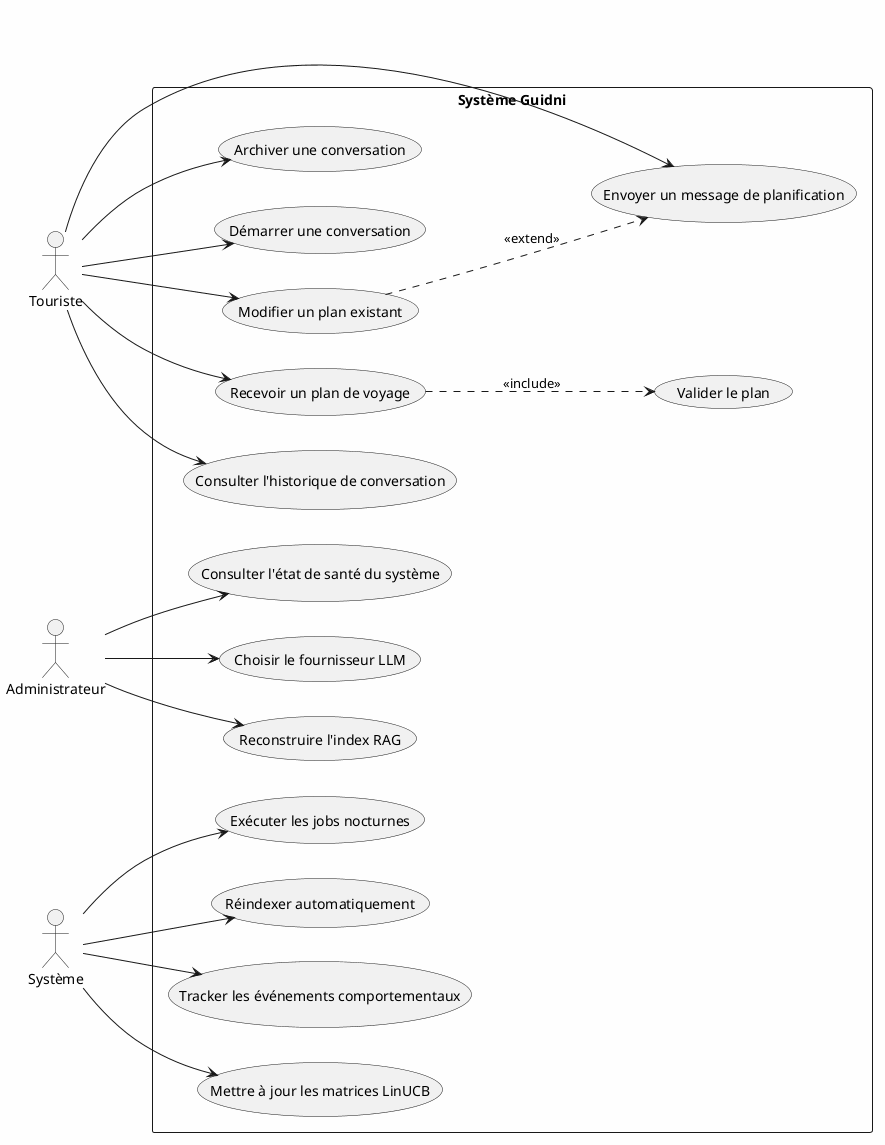
\includegraphics[width=\textwidth]{diagrams/fig_03_use_case_global.png}
    \caption{Diagramme des cas d'utilisation global — Sprint 1}
    \label{fig:sprint1_usecase}
\end{figure}

\subsection{Description textuelle des cas d'utilisation}

Les tableaux suivants décrivent les cas d'utilisation principaux :

\begin{table}[H]
    \centering
    \caption{UC-01 : Consulter l'état de santé du système}
    \label{tab:uc_health}
    \small
    \begin{tabular}{p{2.5cm} p{10cm}}
        \toprule
        \textbf{Champ} & \textbf{Description} \\
        \midrule
        Titre & Consulter l'état de santé du système \\
        Acteur & Administrateur \\
        Pré-condition & L'administrateur est authentifié \\
        Scénario nominal & 
        (1) L'admin accède à GET /health ;
        (2) Le système vérifie la connexion DB ;
        (3) Le système vérifie la disponibilité LLM ;
        (4) Le système vérifie l'état de l'index RAG ;
        (5) Le système retourne un JSON de statut \\
        Post-condition & L'administrateur connaît l'état opérationnel \\
        \bottomrule
    \end{tabular}
\end{table}


% ────────────────────────────────────────────────────────────────
\section{Conception}
% ────────────────────────────────────────────────────────────────

\subsection{Architecture globale}

L'architecture retenue repose sur l'articulation coordonnée de deux sous-systèmes logiciels majeurs s'appuyant sur une base de données PostgreSQL unifiée.

\begin{figure}[H]
    \centering
    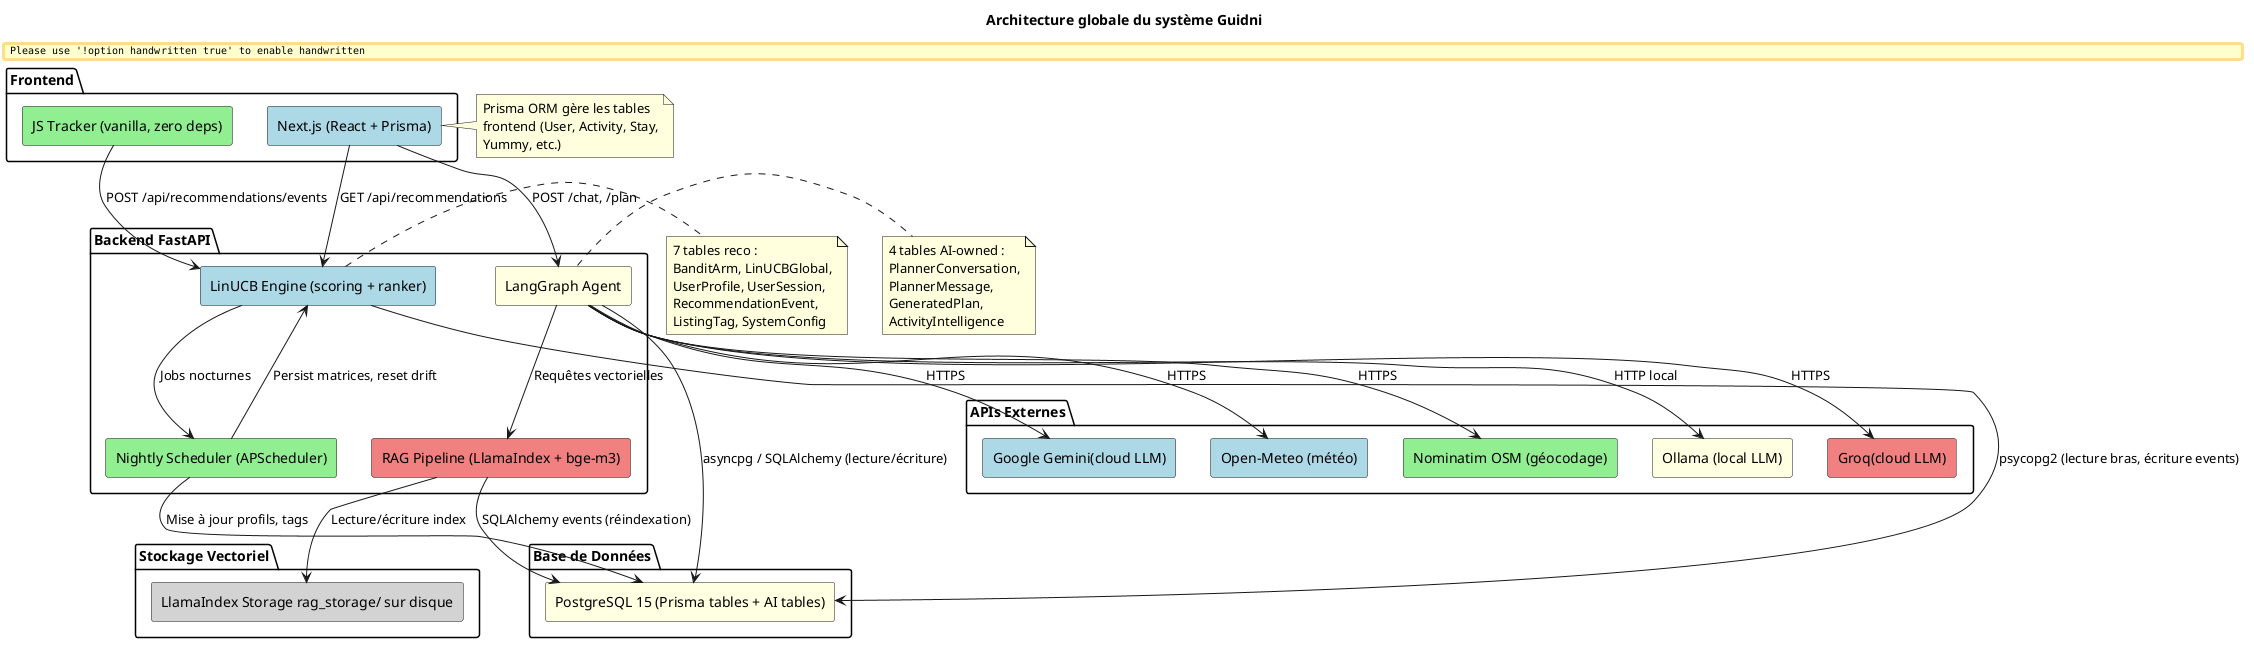
\includegraphics[width=0.95\textwidth]{diagrams/fig_03_global_architecture.png}
    \caption{Architecture globale du système Guidni}
    \label{fig:sprint1_architecture}
\end{figure}

\subsection{Diagramme de séquence — Endpoint Health}

\begin{figure}[H]
    \centering
    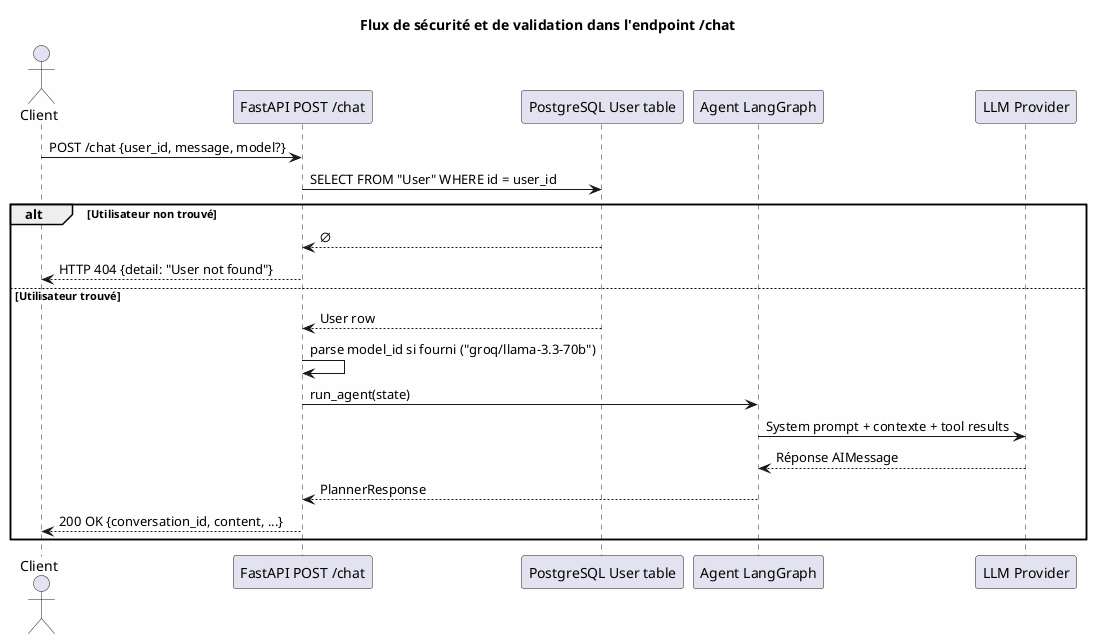
\includegraphics[width=\textwidth]{diagrams/fig_03_security_flow.png}
    \caption{Diagramme de séquence — Vérification de santé}
    \label{fig:sprint1_sequence}
\end{figure}


% ────────────────────────────────────────────────────────────────
\section{Réalisation}
% ────────────────────────────────────────────────────────────────

\subsection{Endpoint GET /health}

L'endpoint de santé a été implémenté avec les checks suivants :
\begin{itemize}
    \item Vérification de la connexion PostgreSQL via asyncpg
    \item Test de disponibilité d'Ollama (si configuré)
    \item Validation de la présence de l'index RAG en mémoire
\end{itemize}

\begin{figure}[H]
    \centering
    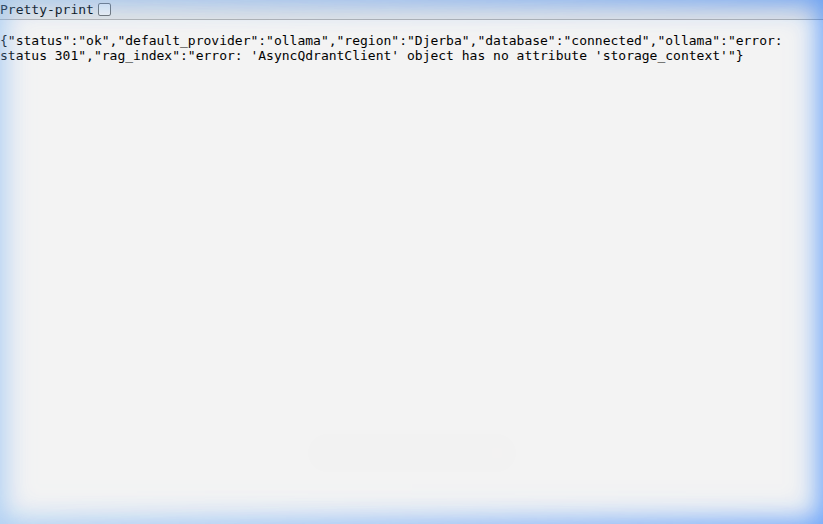
\includegraphics[width=0.8\textwidth]{diagrams/screen_06_health_endpoint.png}
    \caption{Capture d'écran — Response de l'endpoint /health}
    \label{fig:sprint1_health}
\end{figure}

\subsection{Schéma de base de données}

Le modèle de données a été conçu avec les entités suivantes :
\begin{itemize}
    \item User, Conversation, Message (gestion conversations)
    \item Activity, Stay, Restaurant, Attraction (catalogue touristique)
    \item LinUCBGlobal, UserProfile (recommandation)
    \item RAGIndex (index vectoriel)
\end{itemize}


% ────────────────────────────────────────────────────────────────
\section{Sprint Review et Retrospective}
% ────────────────────────────────────────────────────────────────

\subsection{Sprint Review}

À la clôture de ce Sprint inaugural, la phase de Sprint Review s'est orchestrée par un passage en revue détaillé de l'ensemble des propositions architecturales. L'encadrant et Scrum Master, M. Nizar Tenzekhti, a formellement contresigné l'ambition technologique et la justesse du modèle mental binaire (Agent / Bandit Contextuel). Le Product Backlog a été qualifié d'opérationnel pour initier l'itération de développement active.

\subsection{Sprint Retrospective}

La Sprint Retrospective consécutive a permis d'acter une anticipation du risque non négligeable : la gestion hétérogène des flux asynchrones entre les appels base de données et l'imprévisibilité de certaines latences inhérentes aux API des grands modèles de langage. Cette réflexion a mené à renforcer l'intention d'instrumenter le code de façon omniprésente par le truchement de fichiers journaux rigoureux dès l'entame du Sprint 2.


% ────────────────────────────────────────────────────────────────
\section{Conclusion du chapitre}
% ────────────────────────────────────────────────────────────────

L'accomplissement de ce premier Sprint a posé les assises théoriques incontournables au projet Guidni. En cristallisant explicitement les besoins à travers des récits utilisateurs prioritaires et en cartographiant la symbiose attendue d'un agent cognitif LangGraph et d'un moteur LinUCB, nous avons érigé une ligne directrice probante. Les choix de conception actés, se reposant massivement sur la flexibilité asynchrone de Python et de FastAPI, dissipent ainsi les incertitudes algorithmiques fondamentales. Forte de ces directives et de ces outils de traçage, la seconde itération se consacrera inévitablement à l'implémentation logique et sémantique directe de la machine à états de l'agent planificateur, fondation pivotale de l'expérience utilisateur.
